% input files

% \section{Математический анализ I}

Lorem ipsum dolor sit amet, consectetur adipisicing elit, sed do eiusmod
tempor incididunt ut labore et dolore magna aliqua. Ut enim ad minim veniam,
quis nostrud exercitation ullamco laboris nisi ut aliquip ex ea commodo
consequat. Duis aute irure dolor in reprehenderit in voluptate velit esse
cillum dolore eu fugiat nulla pariatur. Excepteur sint occaecat cupidatat non
proident, sunt in culpa qui officia deserunt mollit anim id est laborum.

\begin{figure}[h]
    \centering
    \incfig{1}
    \caption{Первая картинка.}
\end{figure}

Lorem ipsum dolor sit amet, consectetur adipisicing elit, sed do eiusmod
tempor incididunt ut labore et dolore magna aliqua. Ut enim ad minim veniam,
quis nostrud exercitation ullamco laboris nisi ut aliquip ex ea commodo
consequat. Duis aute irure dolor in reprehenderit in voluptate velit esse
cillum dolore eu fugiat nulla pariatur. Excepteur sint occaecat cupidatat non
proident, sunt in culpa qui officia deserunt mollit anim id est laborum.

% document's head
\vspace{2cm}

\begin{center}
    \LARGE \textsc{Конспект второго тома курса теоретической физики <<Теория поля>>}
\end{center}

\hrule

\begin{flushright}
    \begin{tabular}{rr}
    % written by:
        \textbf{Авторы}: 
        & Хоружий Кирилл \\
        & Примак Евгений \\
        &\\
    % date:
        \textbf{От}: &
        \textit{\today}\\
    \end{tabular}
\end{flushright}

\thispagestyle{empty}
\tableofcontents
\newpage

Взаимодействие частиц друг с другом можно описывать с
помощью понятия силового поля.Частица создает вокруг себя поле; на всякую другую частицу, находящуюся в этом поле, действует некоторая сила.

Оказывается, что свойства частицы в отношении ее взаимодействия с электромагнитным полем определяются всего одним параметром -- так называемым зарядом частицы.


\subsubsection*{Уравнение движения пробного заряда}

Как было показано в введение, уравнение движения частицы в электромагнитном поле запишется, как
\begin{equation*}
    \frac{d \vc{p}}{d t} = 
    \underbrace{
        -\frac{e}{c} \frac{\partial \vc{A}}{\partial t} - e 
    }_{
        \text{про } E
    }
    + 
    \underbrace{
        \frac{e}{c} \left[\vc{v} \times \rot \vc{A} \right]
    }_{
        \text{про } H   
    }
\end{equation*}
Так как первая часть не зависит от скорости, то естественно ввести следующие величины
\begin{align*}
    \vc{E} &= -\frac{1}{c} \frac{\partial \vc{A}}{\partial t} - \grad \varphi 
    & \text{--- \textit{напряженность электрического поля}}
    \\
    \vc{H} &= \rot \vc{A} 
    & \text{--- \textit{напряженность магнитного поля}}
\end{align*}
Теперь уравнение движения в ЭМ поле примет вид
\begin{equation}
    \frac{d \vc{p}}{d t} = - e \vc{E} + \frac{e}{c} \left[\vc{v} \times \vc{H} \right]
    \text{\ \ --- \ \ \textit{сила Лоренца}.}
\end{equation}
Таким образом может определить $\vc{E}$, как отношение силы $\vc{F}$, действующей на неподвижный заряд, помещенный в данную точку поля к величине этого заряда $q$: $\vc{E} = \vc{F} / q$. 

\subsubsection*{Теорема Гаусса}

Как было показано в введение, верно что
\begin{equation*}
    \div E = 4 \pi \rho.
\end{equation*}
Или, в интегральной форме, по теореме Стокса
\begin{equation*}
    \int \div \vc{E} \d V = \oint \vc{E} \cdot \d \vc{f} = 4 \pi \int \rho \d V.
\end{equation*}


\subsubsection*{Закон сохранения заряда}
Изменение заряда в объеме в единицу времени:
\begin{equation*}
    \oint \rho \vc{v} \cdot \d \vc{f} = 
     - \frac{\partial }{\partial t} \int \rho \d V,
\end{equation*}
где минус появился из-за выбора направления нормали к поверхности. Это уравнение можно переписать в виде
\begin{equation}
    \frac{\partial }{\partial t} \int \rho \d V = - \oint \vc{j} \cdot \d \vc{f} = - \int \div \vc{j} \d V,
    \hspace{0.25cm} \Rightarrow \hspace{0.25cm} 
    \int \left(
        \div \vc{j} + \frac{\partial \rho}{\partial t} \d V
    \right) = 0,
    \hspace{0.25cm} \Rightarrow \hspace{0.25cm} 
    \boxed{
        \div \vc{j} + \frac{\partial \rho}{\partial t}  = 0
    }.
\end{equation}
Таким образом алгебраическая сумма зарядов электрически замкнутой системы сохраняется. Требование релятивистской инвариантности приводит к тому, что закон сохранения заряда имеет локальный характер: изменение заряда в любом наперёд заданном объёме равно потоку заряда через его границу.


\subsubsection*{Принцип суперпозиции}

Как показывает опыт, электромагнитное поле подчиняется так называемому принципу суперпозиции: поле, создаваемое системой зарядов, представляет собой результат простого сложения полей, которые создаются каждым из зарядов в отдельности. Это значит, что напряженности результирующего поля в каждой точке равны сумме (векторной) напряженностей в этой точке каждого из полей в отдельности.

Всякое решение уравнений поля является полем, которое может быть осуществлено в природе. Согласно принципу суперпозиции сумма любых таких полей тоже должна быть полем,
которое может быть осуществлено в природе, т. е. должно удовлетворять уравнениям поля.

Как известно, линейные дифференциальные уравнения как
раз отличаются тем свойством, что сумма любых его решений
тоже является решением. Следовательно, уравнения для поля
должны быть линейными дифференциальными уравнениями.



\subsubsection*{Закон Кулона}

Рассмотрим точечный заряд, окружим его сферой и запишем для неё теорему Гаусса:
\begin{equation*}
    \oint_{\partial S} \vc{E} \cdot \d \vc{f} = 4 \pi e,
    \hspace{0.5cm} \Rightarrow \hspace{0.5cm} 
    E = \frac{e}{R^2},
    \hspace{0.5cm} \Leftrightarrow \hspace{0.5cm} 
    \vc{E} = \frac{e}{R^2} \frac{\vc{R}}{R}, 
\end{equation*}
что верно в силу радиальной симметрии. Так мы получили \textit{закон Кулона}. 

Потенциал же $\varphi = e / R$, или, для системы зарядов,
\begin{equation*}
    \varphi = \sum_a \frac{e_a}{R_a}, \text{\ \ или \ \ }
    \varphi = \int \frac{\rho}{R} \d V.
\end{equation*}
\textit{Забавный факт}: подстановка в уравнение пуассона приводит к уравнению вида $\Delta (1/R) = -4\pi \cdot \delta(R)$. 

% Простейшим примером системы зарядов является \textit{диполь} $q_1 + q_2 = 0$, для которого верно, что
% \begin{equation}
%     \vc{E} = \frac{q}{r_1^2} \frac{\vc{r}_1}{r_1} - \frac{q}{r_1^2} \frac{\vc{r}_2}{r_2} 
%     \hspace{0.5cm} \overset{l \ll r_2, r_1}{\underset{\Longrightarrow}{}} \hspace{0.5cm} 
%     \vc{E} = \frac{3 (\vc{p} \cdot \vc{n}) \vc{n}}{r^3}  - \frac{\vc{p}}{r^3},
% \end{equation}
% где $\vc{n}$ -- единичный вектор направления к рассматриваемой точке, а $\vc{p}=q \vc{l}$ -- \textit{дипольный момент}.

\subsubsection*{Дипольный момент}


Чуть подробнее остановимся на системе зарядов и дипольном моменте. Рассмотримм поле от системы зарядов на большом расстоянии от этой системы. Выберем начало координат где-то внутри этой системы. В точке, нам интересной, $R_0$ 
\begin{equation*}
    \varphi = \sum_a \frac{e_a}{|\vc{R}_0-\vc{r}_a|}.
\end{equation*}
Нам интересен случай $\vc{R}_0 \gg \vc{r}_0$, так что разложим в ряд до второго члена по $\vc{r}_a/R_0$. Вспомнив, что $f(\vc{R}_0-\vc{r}) \approx f(\vc{R}_0) - \vc{r} \grad f(\vc{R}_0)$ получим
\begin{equation*}
    \varphi = \frac{\sum e_a}{R_0} - \sum e_a \vc{r}_a \grad \frac{1}{R_0}.
\end{equation*}
Теперь естественно ввести \textit{дипольный момент} системы $\vc{p} = \sum_a e_a \vc{r}_a$. Важно, что если $\sum e_a = 0$, то $\vc{d}$ не зависит от выбора начала координат. Действительно:
\begin{equation*}
    \vc{r}_a' = \vc{r}_a + \vc{l},
    \hspace{0.5cm} 
    \vc{d}' = \sum e_a \vc{r}_a' + \vc{l} \sum e_a = \vc{p}.
\end{equation*}
Теперь естественно разделить 
\begin{equation*}
    \vc{d} = \sum e_a^+ \vc{r}_a^+ - \sum e_a^- \vc{r}_a^- = \vc{R}^+ \sum e_a^+ - \vc{R}^- \sum e_a^-, 
    % \hspace{0.5cm} 
    \text{\ \ \ где \ \ \ }
    \vc{R}^+ = \frac{\sum e_a^+ \vc{r}_a^+}{\sum e_a^+}, \ 
    \vc{R}^- = \frac{\sum e_a^- \vc{r}_a^-}{\sum e_a^-}.
\end{equation*}
В случае $\sum e_a^+ = \sum e_a^- = e$, естественно ввести $\vc{R}_{+-} = \vc{R}^+ - \vc{R}^-$, тогда $\vc{d} = e \vc{R}_{+-}$. Потенциал в таком случае
\begin{equation}
    \sigma = - \vc{d} \grad \frac{1}{R_0} = \frac{\vc{d} \cdot \vc{R}_0}{R_0^3},
\end{equation}
тогда $E$
\begin{equation}
    \vc{E} = - \grad \frac{\vc{d} \cdot \vc{R}_0}{R_0^3} = - \frac{1}{R_0^3} \grad \left(\vc{p} \cdot \vc{R}_0 \right) - \left(\vc{p} \cdot \vc{R}_0 \right) \grad \frac{1}{R_0^3},
    \hspace{0.25cm} \Rightarrow \hspace{0.25cm} 
    \boxed{
        \vc{E} = \frac{1}{R_0^3} \left[ \vph
            3 \left(\vc{n} \cdot \vc{p}\right) \vc{n} - \vc{p}
        \right]}, \text{\ \ где \ \ } \vc{n} = \frac{\vc{R}_0}{|R_0|}.
\end{equation}
В частности, выбрав ось $Oz$ по $\vc{p}$, найдём, что
\begin{equation*}
    E_z = \frac{p}{R_0^3} \left(3 \cos^2 \theta - 1\right);
    \hspace{0.5cm} 
    E_x = \frac{p}{R_0^3} \left(3 \sin^2 \theta - 1\right);
\end{equation*}
Или, разбив на радиальную и тангенцальные состовляющие:
\begin{equation*}
    E_R = 2 \frac{p}{R)^3}  \cos \theta, \hspace{0.5cm} 
    E_{\tau} = -2 \frac{p}{R_0^3} \sin \theta.
\end{equation*}

\subsubsection*{\red{Гауссова система единиц (СГС) и система
СИ.}}

\red{
Lorem ipsum dolor sit amet, consectetur adipisicing elit, sed do eiusmod
tempor incididunt ut labore et dolore magna aliqua. Ut enim ad minim veniam,
quis nostrud exercitation ullamco laboris nisi ut aliquip ex ea commodo
consequat. Duis aute irure dolor in reprehenderit in voluptate velit esse
cillum dolore eu fugiat nulla pariatur. Excepteur sint occaecat cupidatat non
proident, sunt in culpa qui officia deserunt mollit anim id est laborum.
} % Закон Кулона и теорема Гаусса
Вместо поиска $\vc{E}$ достаточно найти $\varphi$,
\begin{equation*}
    \left\{\begin{aligned}
        &\vc{E} = -\frac{1}{c}\frac{\partial \vc{A}}{\partial t} - \grad \varphi \\
        &\div \vc{E} = 4 \pi \rho \\
    \end{aligned}\right.
    \hspace{0.5cm} \Rightarrow \hspace{0.5cm} 
    \div \grad \varphi \equiv \Delta \varphi = 
    \left\{\begin{aligned}
        &- 4 \pi \rho &\text{ур. Пуассона} \\
        &\phantom{42} 0 &\text{ур. Лапласа}
    \end{aligned}\right.
\end{equation*}


Как может быть поставлена задача? Заданы граничные значения, найти распределения зарядов. Заданы заряды, найти распределения. Что-то задано, что-то не задано. Во всех трёх случаях \textbf{решение уравнения Пуассона единственно}. 


К слову, так как $\varphi = \varphi(\vc{r})$, а при $A_i = \const$ верно, что $\vc{E} = -\grad \varphi$, то электростатическое поле потенциально. Также это можно увидеть в работе ЭМ сил, при перемещении заряда по замкнутому контуру:
\begin{equation*}
    A_{\text{замкн}}/q = \oint_{(L)} \vc{E} \cdot \d \vc{l} = - \frac{1}{c} \frac{\partial }{\partial t} \int \vc{H} \cdot \d \vc{f} = 0.
\end{equation*}

\vspace{-10pt}

\subsubsection*{Разность потенциалов}

\begin{to_def} 
      Если на участке цепи не действуют сторонние силы, работа по перемещению включает только работу потенциального электрического поля и \textit{электрическое напряжение} $U_{AB}$ между $A$ и $B$ совпадает с разностью потенциалов $\varphi_A - \varphi_B = A^{\text{el}}_{AB}/q$. В общем случае $U_{AB} = \varphi_A - \varphi_B + \mathscr{E}_{AB}$.
\end{to_def}

\subsubsection*{Граничные условия на заряженной поверхности}

\vspace{-10pt}

\begin{minipage}[c]{0.45\textwidth}
\noindent
    По теореме Гаусса верно, что
    \begin{align*}
        E_{2n_2} \cancel{\Delta S} + E_{1n_1} \cancel{\Delta S} &= 4\pi\sigma \cancel{\Delta S}, \\
        E_{2n} - E_{1n} &= 4\pi\sigma
    \end{align*}
\noindent
    По теореме циркуляции верно, что
    \begin{align*}
        E_{2l} \cancel{\Delta} l - E_{1l} \cancel{\Delta} l &= 0 \\
        E_{2l} - E_{1l} &= 0.
    \end{align*}
\end{minipage}
\hfill
\begin{minipage}[c]{0.45\textwidth}
    \incfig{3}
\end{minipage}

\vspace{-10pt}

\subsubsection*{Проводники}

\begin{to_def}[пусть так]
    \textit{Проводник} -- костяк частиц, окруженных \textit{свободными} электронами, которые в пределах тела могут перемещаться на какие угодно
    расстояния. 
\end{to_def}

\vspace{-10pt}

\begin{minipage}[c]{0.55\textwidth}
    В частности, для проводников, верно, что
    \begin{align*}
        E_n &= 4 \pi \sigma \\
        E_\tau &= 0
    \end{align*}
\end{minipage}
\hfill
\begin{minipage}[c]{0.35\textwidth}
    \incfig{4}
\end{minipage}

Собственно, объёмных зарядов в проводнике нет, поверхностные есть и компенсируют внешнее поле. Аналогично работает решетка Фарадея, электростатическое поле не проникает в проводники.


\subsubsection*{Метод изображений}

Если существует некоторая эквипотенциальная поверхность разделяющая пространство на два полупространства, то можем считать что эта поверхность является проводящей. И наоборот, проводящую поверхность можно заменить, на системы зарядов в полупространстве, ей ограниченном, создающих эквипотенциальную поверхность.

 % Теорема о циркуляции для электрического поля. Потенциал.
\section{Проводники}

\begin{to_def}[пусть так]
    \textit{Проводник} -- костяк частиц, окруженных \textit{свободными} электронами, которые в пределах тела могут перемещаться на какие угодно
    расстояния. 
\end{to_def}

\begin{minipage}[c]{0.55\textwidth}
    В частности, для проводников, верно, что
    \begin{align}
        E_n &= 4 \pi \sigma \\
        E_\tau &= 0
    \end{align}
\end{minipage}
\hfill
\begin{minipage}[c]{0.35\textwidth}
    \incfig{4}
\end{minipage}

Собственно, объёмных зарядов в проводнике нет, поверхностные есть и компенсируют внешнее поле. Аналогично работает решетка Фарадея, электростатическое поле не проникает в проводники. % Проводник в электростатическом поле. Дифференциальные соотношения
\subsection{Обращение с обратным образом (?)}

На данный момент у нас есть отображения для $U \in \mathbb{R}^n$ и $V \in \mathbb{R}^k$, считая $U \overset{F}{\longrightarrow} V$

\vspace{-5mm}

\begin{minipage}[t]{0.45\textwidth}
\begin{align*}
    C^{\infty} (U) &\overset{F^*}{\longleftarrow} C^{\infty} (V) \\
    T_P U &\overset{d_P F}{\longrightarrow} T_{F(P)} V
\end{align*}
\end{minipage}
\hfill
\begin{minipage}[t]{0.45\textwidth}
\begin{align*}
    U &\overset{F}{\longrightarrow} V \overset{\varphi}{\to} \mathbb{R} \\
    U &\overset{F^* \varphi}{\longrightarrow} \mathbb{R},
    \hspace{0.5cm} 
    \text{где }
    \hspace{0.5cm} 
    F^* \varphi  \overset{\mathrm{def}}{=} \varphi \circ F,
\end{align*}
\end{minipage}

\vspace{-3mm}

\begin{equation}
    \overbrace{
        d_P F(
            \underbrace{X}_{\in T_P U}
            )
    }^{\in T_{F(P)} V}
    \underbrace{\varphi}_{\in C^{\infty} (V)} 
    =
    X 
    \underbrace{F^* \varphi}_{\in C^\infty (U)}.
\end{equation}

С формами ситуация схожая с функциями, то есть
$$
    C^\infty (V) = \Gamma^0 (V),
$$
получается
\begin{align*}
    \Omega^k (U) \overset{F^*}{\longleftarrow} \Omega^k (V), \\
    T_U U \overset{d_P F}{\longrightarrow} T_{F(P)} (V).
\end{align*}
Теперь пусть $X_1, \ldots, X_k$ -- векторное поле на $U$, тогда
$$
    (F^* \omega) (X_1, \ldots, X_k) = \omega\left(
        d F(X_1), \ldots, d F(X_k)
    \right).
$$
Собственно, факт:
\begin{equation}
    d F^* \omega = F^* \d \omega.
\end{equation}
И ещё факт
\begin{equation}
    F^* (\sigma \wedge \tau) = F^* \sigma \wedge F^* \tau.
\end{equation}



%%%%%%%%%%%%%%%%%%%%%%%%%%%%%%%%%%%%%%%%%%%%%%%%%%%%%%%%%%%%%%%%%%%%%%%%%%%%%%%%%%%
\subsection{Плоские кривые}
Кривые должны быть гладкими, но этого недостаточно. Поэтому требуем и \textit{регулярность}:
\begin{equation}
    \forall x, y \colon F(x, y) = 0
    \hspace{0.5cm} 
    \left(
        \frac{\partial F}{\partial x}, \frac{\partial F}{\partial y} 
    \right) \neq (0, 0),
\end{equation}
а в параметрическом задание
\begin{equation}
    \forall t \in (a, b)
    \hspace{0.5cm} 
    \dot{\vc{r}} (t) = (\dot{x} (t), \dot{y}(t)) \neq (0, 0).
\end{equation}

Пусть $F(x, y) = 0$ -- регулярная гладкая неявно заданная кривая. Тогда в окрестности любой своей точки её можно задать как регулярную гладкую параметрическую кривую. 




 % Метод изображений. Ёмкость. Электрическое поле в веществе
% \section{Электрическое поле в веществе}

\begin{to_def} 
    \textit{Диэлектрик} -- совокупность заряженных частиц в вакууме, без свободного заряда. Все заряды <<привязаны>> к частицам, однако может возникать избыточный заряд.
\end{to_def}

Немного поправим\footnote{
    Ещё раз, почему возникают поляризационные заряды? Потому что мы достаточно далеко разнесли состовялющие некогда нейтральной частицы?
} теорему Гаусса:
$$
    \oint_S E_n \d S = 4\pi (q + q_{\text{пол}})
$$
Введём вектор поляризованности
$$
    \vc{P} = \frac{1}{\Delta V} \sum_{\Delta V} \vc{p}_i.
$$
Или, говоря о поверхностных зарядах:
$$
    P_n = \sigma_{\text{пол}}, \hspace{0.5cm} \oint_S P_n \d S = - q_{\text{пол}}.
$$
Тогда
\begin{equation}
    \oint_S
    \underbrace{\left(\vc{E} + r\pi \vc{P} \right)}_{\vc{D}}
    \d S = 4\pi q 
\end{equation}
Ну и, не забывая о циркуляции,
$$
    \oint_L E_l \d l = 0.
$$
А рассматривая класс линейных диэлектриков $\vc{P} = \alpha \vc{E}$, получим, что
$$
    \vc{D} = \vc{E} (\underbrace{1 + 4 \pi \alpha}_{\varepsilon}),
$$
где
$
    \alpha \text{ -- коэффициент поляризации},$ $
    \varepsilon \text{ -- диэлектрическая проницаемость}.
$



\subsubsection*{Граничные условия на границе двух диэлектриков}

Для границы, рассмотрев область без свободных зарядов, с учётом теормы Гаусса, можно записать, что $D_{1n} = D_{2n}$, или
$$
    \varepsilon_1 E_{1n} = \varepsilon_2 E_{2n},
$$
или
$$
    E_{2n} - E_{1n} = 4 \pi \sigma_{\text{пол}}.
$$

Посмотрим на тангенсальную состовляющую. Рассмотрим вытянутый прямоугольник вдоль границы, тогда получим, что
$$
    E_{1\tau} = E_{2\tau}.
$$

\subsubsection*{Плоский конденсатор}


Рассмотрим плоский конденсатор, засунем в него диэлектрическую пластинку. Возникнут поляризационные заряды, тогда
$$
    \vc{D}_1 = \vc{D}_2 = E_0 = 4\pi\sigma.
$$
Поле внутри диэлектрика тогда
$$
    E_2 = \frac{4\pi\sigma}{\varepsilon}; \hspace{0.5cm} 
    E_1 - E_2 = 4\pi\sigma\left(1- \frac{1}{\varepsilon} \right)  = 4\pi\sigma_{\text{пол}}
    \hspace{0.5cm} \Rightarrow \hspace{0.5cm} 
    \sigma_{\text{пол}} = \sigma \frac{\varepsilon-1}{\varepsilon}.f
$$


\subsubsection*{Поле системы зарядов в диэлектрике}
По теореме Гаусса
$$
    D \cdot 4\pi r^2 = 4 \pi q, \hspace{0.25cm}  D = \varepsilon E
    \hspace{0.5cm} \Rightarrow \hspace{0.5cm} 
    E = \frac{q}{\varepsilon r^2} 
$$
По принципу суперпозиции
$$
    \vc{E} = \sum \vc{E}_i = \sum \frac{\vc{E}_{i0}}{\varepsilon} 
    = \frac{\vc{E}_0}{\varepsilon} .
$$
Но только для линейной поляризации.

Получается, для конденсатора верно, что при заполнение онного диэлектриком, напряжение $U_0$ изменится так, что
$$
    U =  \frac{U_0}{\varepsilon} , \hspace{0.5cm} C = \frac{q}{U} 
    \hspace{0.25cm} \Rightarrow \hspace{0.25cm} C = \varepsilon C_0.
$$  

 % Электрическое поле в веществе–2, энергия электрического поля
\subsection{Производная по направлению}

Раньше определили
$$
    \partial_V f(A) = \lim_{\varepsilon \to 0} \frac{f(A + \varepsilon V) - f(A)}{\varepsilon},
$$
но сложность в том, что $A + \varepsilon V \notin \Sigma$. 
Но гладкую функцию с поверхности может всегда продлить в некоторую окрестность поверхности. Это продолжение $F$ не единственно. 

\begin{to_def} 
    Определим
    $$
         \partial_V f(A) \overset{\mathrm{def}}{=} \partial_V F(A),
    $$ 
    при чём def инвариантно к выбору $F$.
\end{to_def}

\begin{proof}[$\triangle$]
    \begin{minipage}[t]{0.9\textwidth}
        \begin{enumerate}[label = \Roman*.]
            \item Мы дифференцируем только вдоль касательных векторов к $\Sigma$, следовательно существует кривая $\gamma$ на $\Sigma$ такая, что
            \begin{align*}
                &1) \ \forall t \; \gamma(t) \in \Sigma \\
                &2) \ \gamma(0) = A \\
                &3) \ \ddot{\gamma}(0) = V.
            \end{align*}
            \item Тогда
            $$
                \underbrace{\frac{d}{dt} f(\gamma(t)) \bigg|_{t=0}}_{
                *
                } = 
                \frac{d}{dt} F(\gamma(t)) \bigg|_{t=0} =
                \frac{\partial F}{\partial x^i} (\set{x}{n}) \dot{x}^i (t) \bigg|_{t=0} =
                \frac{\partial F}{\partial x^i} (A) V^i = 
                \underbrace{\partial_V F(A)}_{
                **
                }
                ,
            $$
            считая $\gamma(t) = [x^1(t),\ldots, x^n(t)]$.
            \item Но, т.к. $*$ не зависит от выбора $F$, то и $**$ не зависит от выбора $F$. Тогда $\partial_V f(A)$ определена корректно.
            \item К слову, $**$ не зависит от выбора пути, тогда и $*$ не зависит от выбора пути.
        \end{enumerate}
    \end{minipage}

\phantom{42}
\end{proof}

Получается мы можем определить понятие  дифференцирования гладкой функции на поверхности в точке.

\begin{to_def} 
     Для $f\colon \Sigma \to \mathbb{R}$ достаточно быть определенной в некоторой окрестности точки $A$. Скажем, что $D$ -- дифференцирование на $\Sigma$ в точке$A$, если
    \begin{align*}
        &1) \ Df \in \mathbb{R} \\
        &2) \ D(f+g) = Df + Dg \\
        &3) \ D(fg) = (Df) \cdot g(A) + f(A) \cdot (Dg).
    \end{align*}
    Пусть $\set{u}{k}$ -- локальные координаты в окрестности точки $A$.
\end{to_def}


\begin{to_lem} 
     Для $\forall D \ \exists \set{V}{K}$ такой, что
     $$
         Df = \frac{\partial f}{\partial u^i} (A) V^i.
     $$
\end{to_lem}

Пусть есть некоторый касательный вектор $W \in T_A \Sigma$
$$
    W = W^i r_{u^i} (A).
$$
Тогда можно рассматривать путь $\gamma(t)$ в локальных координатах такой, что
$
    \gamma(0) = A, \ \dot{\gamma}(0) = W,
$
то есть для $A = (\set{u_0}{k})$ и $\gamma(t) = \left[
    u^1(t), \ldots, u^k(t)
\right]$ верно, что
$$
    u^i(0) = u^i_0, \hspace{0.5cm} \dot{u}^i(0) = W^i.
$$
Тогда
$$
    \partial_W f(A) = \frac{d}{dt} f(\gamma(t)) \bigg|_{t=0}
    =
    \frac{\partial f}{\partial u^i} (A) \ W^i.
$$

Получается, что \textbf{каждый} касательный вектор $W$ даёт дифференцирование $\partial_W \big|_A$, и \textbf{каждое} дифференцирование в $A$ получается из касательного вектора. Поэтому будем писать просто
\begin{equation}
    \boxed{
    W = \partial_W = W^i \frac{\partial }{\partial u^i} .
    }
\end{equation}


\subsection{Двойственность}

Раз есть касательные векторы, то есть и кососимметрические полилинейные функии на них. 
Так приходим к следующей двойственной структуре:

$\cdot$ $T_P \Sigma$ -- \textit{касательное пространство} к $\Sigma$ в $P$,

$\cdot$ $T_P^* \Sigma \overset{\mathrm{def}}{=}  \left(T_P \Sigma\right)^*$ -- \textit{кокасательное пространство} к $\Sigma$ в $P$.

\noindent
Получаются векторное поле $X$: $X(P) \in T_P \Sigma$, и ковекторное поле $\xi$:
$\xi (P) \in T_P^* \Sigma$.

Если $\set{u}{k}$ -- локальные координаты на $\Sigma$, то
$$
    \frac{\partial }{\partial u^i} = r_{u^i}
    \hspace{0.5cm} \text{---} \hspace{0.5cm} 
    \text{базис в } T_P \Sigma.
$$
Соответственно,
$$
    du^1, \ldots, du^k
    \hspace{0.5cm} \text{---} \hspace{0.5cm} 
    \text{базис в } T_P^* \Sigma.
$$
А вот
$$
    \underset{ i_1 < \ldots < i_q}{ du^{i_1} \wedge \ldots \wedge du^{i_q}}
    \hspace{0.5cm} \text{---} \hspace{0.5cm} 
    \text{базис в } \Lambda^q T_P^* \Sigma,
$$
где $\Lambda^q T_P^* \Sigma$ -- пространство $q$-форм.


 % энергия электрического поля
\sbsnum{20}{Интегрирование диф-формы объёма}
Естественно ввести \textit{тензор электромагнитного поля}:
\begin{equation}
{F}_{ik} = 
    \begin{pmatrix}
        0    & E_x & E_y  & E_z   \\
        -E_x  & 0    & -B_z & B_y   \\
        -E_y & B_z  & 0    & -B_x  \\
        -E_z & -B_y & B_x & 0     \\
    \end{pmatrix}_{ik},
    \hspace{2cm} 
{F}^{ik} = 
    \begin{pmatrix}
        0    & -E_x & -E_y  & -E_z   \\
        E_x  & 0    & -B_z & B_y   \\
        E_y & B_z  & 0    & -B_x  \\
        E_z & -B_y & B_x & 0     \\
    \end{pmatrix}^{ik}
\end{equation}
Тогда уравнения Максвелла запишутся в виде
\begin{equation}
    \boxed{
        \varepsilon^{iklm} \partial_k F_{lm} = 0, \hspace{0.5cm} 
        \partial_k F^{ik} = - \frac{4\pi}{c} j^i
    },
\end{equation}
где $j^i = (\rho c, \vc{j})$. Прямой подстановкой тензора ЭМ поля нетрудно убедиться, что

\phantom{42}

\noindent
\begin{minipage}[t]{0.45\textwidth}
\noindent
Дифференциальная форма в СГС:
    \begin{align}
        \vphantom{\oint }
        \div \vc{D} &= 4 \pi \rho \\
        \vphantom{\oint }
        \div \vc{B} &= 0 \\
        \vphantom{\oint }
        \rot \vc{E} &= -\frac{1}{c} \frac{\partial \vc{B}}{\partial t}  \\
        \vphantom{\oint }
        \rot \vc{H} &= \frac{4\pi}{c} \vc{j} + \frac{1}{c} \frac{\partial \vc{D}}{\partial t} 
    \end{align}
\end{minipage}
\hfill
\begin{minipage}[t]{0.45\textwidth}
Интегральная форма в СГС:
    \begin{align}
       \oint \vc{D} \cdot d \vc{s} &= 4\pi Q \\
       \oint \vc{B} \cdot d \vc{s} &= 0 \\
       \oint \vc{E} \cdot d \vc{l} &= - \frac{1}{c} \frac{d}{dt} \int \vc{B} \cdot d \vc{s} \\
        \oint \vc{H} \cdot \d \vc{l} &= \frac{4\pi}{c} I + \frac{1}{c} \frac{d}{dt} \int \vc{D} \cdot \d \vc{s}.
    \end{align}
\end{minipage}

\begin{description*}
    \item[$\vc{E}$]  --- напряженность электрического поля;
    \item[$\vc{H}$]  --- напряженность магнитного поля;
    \item[$\vc{D}$]  --- электрическая индукция;
    \item[$\vc{B}$]  --- магнитная индукция.
\end{description*}

\subsubsection*{Материальные уравнения}

В проводниках связь между плотностью тока и напряжённостью электрического поля выражается в линейном приближении \textit{законом Ома}:
\begin{equation*}
    \vc{j} = \sigma \vc{E},
\end{equation*}
где $\sigma$ -- \textit{удельная проводимость среды}.

В среде сторонние электрические и магнитные поля вызывают поляризация $\vc{P}$ и намагничивание вещества $\vc{M}$.
Тогда
\begin{align*}
    \rho_\text{b} &= - \nabla \cdot \vc{P} \\
    \vc{j}_\text{b} &= c \nabla \times \vc{M} + \frac{\partial \vc{P}}{\partial t} ,
\end{align*}
Далее, по определению
\begin{align*}
    \vc{D} &= \vc{E} + 4\pi \vc{P}, &\vc{B} &= \vc{H} + 4 \pi \vc{M} \\
\end{align*}
Что в случае линейной поляризации или линейной намагничиваемости можно записать, как  
$$
    \left\{\begin{aligned}
        \vc{P} &= \chi_{\text{e}} \vc{E}, \\
        \vc{M} &= \chi_{\text{m}} \vc{H}, \\
    \end{aligned}\right.
    \hspace{0.5cm} \Rightarrow \hspace{0.5cm} 
    \left\{\begin{aligned}
         \vc{D} &= \varepsilon \vc{E} = (1 + 4\pi \chi_{\text{e}}) \vc{E}, \\
       \vc{B} &= \mu \vc{H} = (1 + 4 \pi \chi_{\text{m}}) \vc{H}.
    \end{aligned}\right.
$$
где $\varepsilon$ -- \textit{\sout{относительная} диэлектрическая проницаемость}, $\mu$  — \textit{относительная магнитная проницаемость}, $\chi_{\text{e}}$  -- \textit{диэлектрическая восприимчивость}, $\chi_{\text{m}}$ -- \textit{магнитная восприимчивость}.

Наконец, в однородных средах верно, что
\begin{equation*}
    \left\{\begin{aligned}
        \div \vc{E} &= 4\pi \frac{\rho}{\varepsilon},  \\
        \div \vc{B} &= 0,
    \end{aligned}\right.
    \hspace{1cm} 
    \left\{\begin{aligned}
        \rot \vc{E} &= - \frac{1}{c} \frac{\partial \vc{B}}{\partial t}, \\
        \rot \vc{B} &= \frac{4\pi}{c} \mu \vc{j} + \frac{\varepsilon \mu}{c} \frac{\partial \vc{E}}{\partial t},
    \end{aligned}\right.
\end{equation*}
где в оптическом диапазоне принято $n = \sqrt{\varepsilon \mu}$.

\subsubsection*{Граничные условия}
Опять же, в СГС,
\begin{equation*}
    \left\{\begin{aligned}
        (\vc{E}_1 - \vc{E}_2) \times \vc{n}_{1,2} &= 0, \\
        (\vc{H}_1 - \vc{H}_2) \times \vc{n}_{1,2} &= \frac{4\pi}{c} \vc{j}_\text{s},
    \end{aligned}\right.
    \hspace{1cm} 
    \left\{\begin{aligned}
        \left(\vc{D}_1 - \vc{D}_2\right) \cdot \vc{n}_{1,2} &= - 4\pi \rho_\text{s}, \\
        \left(\vc{B}_1 - \vc{B}_2\right) \cdot \vc{n}_{1, 2} &= 0,
    \end{aligned}\right.
\end{equation*}
где $\rho_{\text{s}}$ -- поверхностная плотность свободных зарядов, $\vc{j}_\text{s}$ -- плотность поверхностных свободных токов вдоль границы. 

Эти граничные условия показывают непрерывность нормальной компоненты вектора магнитной индукции, и непрерывность на границе областей тангенциальных компонент напряжённостей электрического поля. 

\subsubsection*{Уравнение непрерывности}

Источники полей $\rho, \vc{j}$ не могут быть заданы произвольным образом. Применяя операцию дивергенции к четвёртому уравнению (закон Ампера—Максвелла) и используя первое уравнение (закон Гаусса), получаем уравнение непрерывности
\begin{equation*}
    \nabla \cdot \vc{j} + \frac{\partial \rho}{\partial t} = 0,
    \hspace{0.5cm} \Leftrightarrow \hspace{0.5cm} 
    \oint_S \vc{j} \cdot \d \vc{s} = - \frac{d }{d t} \int_V \rho \d V.
\end{equation*}




\sbsnum{21}{Представление диф-формы в каноническом виде}
\begin{to_lem} 
\label{lem_6.100}
    Пусть $U = \prod_{i=1}^n (a_i, b_i)$, где $(a_i, b_i) \ni 0$. Пусть $\varphi \colon \mathbb{R} \mapsto \mathbb{R}^+$ -- гладкая функция с компактным носителем, содержащимся в каждом $(a_i, b_i)$, и с единичным интегралом. Для всякой $\nu \in \Omega_{\text{c}}^n (U)$ найдётся число $I$ и форма $\lambda \in \Omega_{\text{c}}^{n-1}(U)$, такие что
    $\nu = I \varphi(x_1) \ldots \varphi(x_n) dx_1 \wedge \cdots \wedge dx_n + d \lambda$.
\end{to_lem}


\begin{to_con} 
\label{con_6.101}
    Пусть $U = \prod_{i=1}^{n} (a_i, b_i)$ -- произведение интервалов. Факторпространство $\Omega_{\text{c}}^n(U) / d \Omega_{\text{c}}^{n-1} (U)$ одномерно. Получается, что всевозможные способы определить интеграл формы $\nu \in \Omega_{\text{c}}^n (U)$ так, чтобы интеграл от $d \lambda$ равнялся нулю, могут отличаться только умножением на константу. \red{Ещё раз.} 
\end{to_con}

\sbsnum{22}{Поведение интеграла от формы при линейной замене координат}

\begin{to_lem}[Поведение интеграла формы при линейной замене координат]
     Интеграл дифференциальной формы $\nu \in \Omega_{\text{c}}^n (\mathbb{R}^n)$ при отображении $A^*$, соответствующем линейному преобразованию $A : \mathbb{R}^n \mapsto  \mathbb{R}^n$ меняет или не меняет знак в зависимости от знака определителя $\det A$, то есть
     \begin{equation*}
         \int_{\mathbb{R}^n} A^* \nu = (\sign \det A) \int_{\mathbb{R}^n} \nu.
     \end{equation*}
\end{to_lem}


\sbsnum{23}{Гладкое разбиение единицы}
\subsubsection*{Давление света}
При полном поглощении запишем следующее:
\begin{equation*}
    w = \frac{E^2}{4\pi} = pc, \hspace{0.5cm} p = \frac{E^2}{4\pi c} 
    \hspace{0.5cm} \Rightarrow \hspace{0.5cm} 
    P = \frac{1}{dS} \frac{d (p\d V)}{d t} = \frac{E^2}{4\pi},
    \hspace{0.5cm} 
    \langle P\rangle = \frac{\langle E^2\rangle}{4\pi}.
\end{equation*}
Или, по-другому
\begin{equation*}
    \left\{\begin{aligned}
        \frac{\partial \vc{E}}{\partial z} &= \rot \vc{E} = - \frac{1}{c} \frac{\partial \vc{H}}{\partial t}, \\
        \frac{\partial \vc{H}}{\partial z} &= \rot \vc{H} = \frac{4\pi}{c} \vc{j} + \frac{1}{c} \frac{\partial E}{\partial t}.
    \end{aligned}\right.
    \hspace{0.5cm} \Rightarrow \hspace{0.5cm} 
    \frac{\partial }{\partial z} \left(\frac{E^2+H^2}{8\pi} \right) = - \frac{1}{c} \frac{\partial \vc{H}}{\partial t} \cdot \frac{\vc{E}}{4\pi}  + \frac{4\pi}{c} \vc{j} \cdot \frac{\vc{B}}{4\pi} + \frac{1}{c} \frac{\partial \vc{E}}{\partial t} \frac{\partial \vc{H}}{\partial 4\pi} = \vc{f} + \frac{1}{8\pi c} \frac{\partial }{\partial t} \left(\vc{E} \cdot \vc{H}\right).
\end{equation*}
Таким образом
\begin{equation*}
    \frac{\partial }{\partial z} 
    \vph
    \langle w\rangle= \langle f \rangle
    \hspace{0.5cm} \Rightarrow \hspace{0.5cm} 
    \langle P\rangle = \int_0^{\infty} \langle f\rangle\d z = w(0) - w(\infty) = w(0) = \frac{\langle E^2\rangle}{4\pi}.
\end{equation*}
Что и требовалось доказать!) Кстати,
\begin{equation*}
\overline{S} = c \cdot \overline{\mathcal W_{\text{эл}}}, \hspace{0.5cm} \Rightarrow \hspace{0.5cm} 
    \vc{g}_{\text{эм}} = \frac{1}{c^2} \vc{S} = \frac{1}{4\pi c} \left[
        \vc{E} \times \vc{H}
    \right].
\end{equation*}

\subsubsection*{Формулы Снеллиуса}

Скорость распространения света
\begin{equation*}
    n = \frac{c}{v} = \sqrt{\varepsilon \mu}.
\end{equation*}
Для нормальной и тангенциальной компоненты воспользуемся граничными условиями
\begin{align*}
    E_2 \cos \psi &= E_1 \cos \varphi - E_1' \cos \varphi \\
    \varepsilon_2 E_2 \sin \psi &= \varepsilon_1 \left(
        E_1 \sin \varphi + E_1' \sin \varphi'
    \right),
\end{align*}
при чём $\varepsilon_2 = n_2^2$. И для $B$ верно, что
\begin{equation*}
    B_1 + B_1' = B_2.
\end{equation*}
Верно, что на границе
\begin{equation*}
    \vc{k} \cdot \vc{r} = k x \sin \varphi,
    \hspace{0.5cm} \Rightarrow \hspace{0.5cm} 
    \vc{E}_1 = \vc{E}_{10} e^{i\omega t} e^{-ik_1 x \sin \varphi},
    \hspace{0.5cm} \Rightarrow \hspace{0.5cm} 
    E_1 \sim \cos (k_1 x \sin \varphi).
\end{equation*}
Вспомним, что $\sqrt{\varepsilon} E = H \sqrt{\mu} = H$, тогда
\begin{equation*}
    \boxed{n_1 (E_1 + E_1') = n_2 E_2}, \hspace{0.5cm} 
    \boxed{
        \varphi = \varphi'
    }.
\end{equation*}
Можем сказать, что
\begin{equation*}
    n_1 \left(
        \hat{E}_{10} e^{ik_1 x\sin \varphi} + \hat{E}_{10} e^{-ik_1' x \sin \varphi' }
    \right) = 
    n_2 \hat{E}_{20} e^{i k_2 x \sin \psi}.
\end{equation*}
Мы знаем связь для $k = 2\pi / \lambda$, соответсвенно $k_1 = k_1'$.  Приходим к системе
\begin{equation*}
        k_1 \sin \varphi = k_2 \sin \psi, \hspace{0.5cm} 
    \frac{n_1 (\hat{E}_{10} + \hat{E}_{10}')}{n_2 \hat{E}_{20}} = \exp\left(
        -ix(
        \underbrace{k_2 \sin \psi - k_1 \sin \varphi}_{=0}
        )
    \right).
\end{equation*}
Ещё можем записать, что
\begin{equation*}
    n = \frac{\varepsilon \mu \omega}{c k}.
\end{equation*}
Получили формулы Снеллиуса.
\begin{equation*}
    \boxed{
        n_1 \sin \varphi = n_2 \sin \psi = \frac{n^2 \omega}{ck} .
    }
\end{equation*}


% \subsubsection*{Формулы Френе}

Запишем формулы Френе. Для $P$-поляризации
\begin{equation*}
    E_2 = E_1 \cdot \left(
        \frac{2 \sin \psi \cos \varphi}{\sin(\varphi + \theta)\cos (\varphi - \psi)} 
    \right),
    \hspace{1cm} 
    E_1' = E_1 \cdot \left(
    \frac{\tg(\varphi - \psi)}{\tg(\varphi + \psi)} 
    \right).
\end{equation*}
Для $S$-поляризации
\begin{equation*}
    E_1' = -E_1 \frac{\sin(\varphi-\psi)}{\sin(\varphi+\psi)},
    \hspace{1cm} 
    E_2 = E_1 \frac{2 \sin \psi \cos \varphi}{\sin(\varphi+\psi)}.
\end{equation*}

При угле между $\vc{k}'$ и $\vc{k}_2$ равным $\pi/2$ волна полностью проникает внутрь. 
Что ж, действительно, $\varphi + \psi = \pi/2$, тогда $n_1 \sin \varphi = n_2 \sin \psi = n_2 \cos \varphi$, тогда $\tg \varphi = n_2 / n_1$.

% \begin{equation*}
%     \varepsilon_2 \sin \psi E_{20} \cos \left(k_2 x \sin \psi \right) = 
%     \varepsilon_1 \left(
%         E_{10} \sin \varphi \cdot \cos \left(
%             k_1 x \sin \varphi
%         \right) + 
%         E_{10}' \sin \varphi' \cos \left(k_1 x \sin \varphi\right)
%     \right)
% \end{equation*}

\subsubsection*{Излучение диполя}

Рассмотрим антенку-диполь, $l \ll \lambda$. Два шарика перезаряжаются, и 
\begin{equation*}
    p = ql = p_0 \cos \omega t.
\end{equation*}
Ток будет равным
\begin{equation*}
    I = \dot{q} = \frac{\dot{p}}{l} = -\frac{1}{l} \omega p_0 \sin \omega t =I_0 \sin \omega t 
    .
\end{equation*}
Окружим диполь сферой. При $r \ll \lambda$ можем пренебречь запаздыванием, тогда можем говорить про статические формулы и $E \sim r^{-3}$ и $B \sim r^{-2}$. 

Однако наиболее интересен второй случай при $r \gg \lambda$. Тогда поле имеет вид сформировавшейся бегущей волны $\vc{k} \nparallel \vc{r}$. Вектор $\vc{E}$ ориентирован по меридиану сферы, вектор $\vc{B}$ ориентирован по широте, $\vc{E}, \vc{B}, \vc{k}$ образуют правую тройку. 
\begin{equation}
    E = B = \frac{
        \ddot{p} \left(t - \frac{r}{c}\right) \sin \theta
    }{
        c^2 r
    }.
\end{equation}
Рассмотрим это подробнее. 
\begin{equation*}
    \ddot{p}\left(t - \frac{r}{c} \right) = \omega_0^2 p_0 \cos \left(
        \omega \left(t - \frac{r}{c} \right)
    \right),
    \hspace{0.5cm} \Rightarrow \hspace{0.5cm} 
    \ddot{p} = - \omega^2 p_0 \cos (\omega t - kr).
\end{equation*}
Найдём среднее значение для вектора Пойтинга
\begin{equation*}
    \overline{S} = \frac{1}{8\pi} E_0^2 n,
    \hspace{0.5cm} \Rightarrow \hspace{0.5cm} 
    \overline{S} = \frac{1}{8\pi c^3} \frac{p_0^2 \omega^4 \sin^2 \theta}{r^2}.
\end{equation*}
Найдём интеграл по поверхности -- полный поток энергии
\begin{equation*}
    \int \overline{S} \d \sigma  = \int \overline{S} 
    2 \pi r \sin \theta r \d \theta = \frac{p_0^2 \omega^4}{3 c^3} 
    =
    \frac{l^2 \omega^2}{3 c^3}  I_0^2.
    =
    \frac{1}{2} R_{\text{изл}} I_0^2.
    .
\end{equation*}





% Для проводник верен закон Ома $\vc{j} = \sigma \vc{E}$, тогда по силе Лоренца
% \begin{equation*}
%     \vc{f} = \frac{1}{c} \left[
%         \vc{j} \times \vc{B}
%     \right] = \frac{1}{c} \left[\sigma \vc{E} \times \vc{B}\right]
%     ,
%     \hspace{0.5cm} \Rightarrow \hspace{0.5cm}

% \end{equation*}











\sbsnum{24}{Поведение интеграла от формы при гладкой замене координат}
Длинная линия — модель линии передачи, продольный размер (длина) которой превышает длину волны, распространяющейся в ней. Такая линия передачи может быть охаракетризована погонными параметрами:
$R_0$ -- погонное сопротивление, $G_0$ -- паразитная, погонная проводимость, $L_0$ -- погонная индуктивность, $C_0$ -- погонная емкость.


Рассмотрим два рядом идущих длинных провода (коаксиальный кабель, например). Тогда в $z$ и $z+ \Delta z$ ток будет различным, как и, соответсвенно, разность потенцаилов. 
\begin{equation*}
    V(z+\Delta z) - V(z) = \frac{L_0 \Delta z}{c^2} \frac{\partial I}{\partial t},
    \hspace{1cm} 
    I(z) = I(z+\Delta z) + \frac{\partial q}{\partial t},
    \hspace{1cm} 
    q = C_0 \Delta z V.
\end{equation*}

\begin{figure}[h]
    \centering
    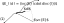
\includegraphics[width=0.25\textwidth]{img/2.png}
    %\caption{}
    %\label{fig:}
\end{figure}

\noindent
Из этих уравнений легко получить, что
\begin{equation}
    \left\{\begin{aligned}
        \frac{\partial U}{\partial z} &= - \frac{L_0}{c^2} \frac{d I}{d t} \\
        \frac{\partial I}{\partial z} &= - C_0 \frac{\partial U}{\partial t} 
    \end{aligned}\right.
    \hspace{0.5cm} \Rightarrow \hspace{0.5cm} 
    \boxed{
        \frac{\partial^2 U}{\partial t^2}  = \frac{c^2}{L_0 C_0} - \frac{\partial^2 V}{\partial z^2} 
    }.
\end{equation}
Решение аналогично будем искать в виде
\begin{equation}
    V = f_1 (z - vt) + f_2 (z + vt),
    \hspace{0.5cm} \Rightarrow \hspace{0.5cm} 
    v = \frac{c}{\sqrt{L_0 C_0}}.
\end{equation}
Кстати, если это всё посчитать для коаксиального кабеля, то
\begin{equation*}
    L_0 = 2 \mu \ln \frac{R_2}{R_1} , \hspace{0.5cm} 
    C_0 = \frac{\varepsilon}{2 \ln \frac{R_2}{R_1} },
    \hspace{0.5cm} \Rightarrow \hspace{0.5cm} 
    v = \frac{c}{\sqrt{\mu \varepsilon}}.
\end{equation*}


\subsubsection*{Коэффициент стоячей волны (standing wave ratio)}
Коэффициент стоячей волны -- отношение наибольшего значения амплитуды напряжённости электрического или магнитного поля стоячей волны в пучностях линии передачи к амплитуде в узлах.
КСВ является мерой согласования нагрузки (например, антенны) с линией передачи.

Наибольшее и наименьшее значения амплитуды соответсвенно равны
\begin{equation*}
    A_{\text{max}} = A_{\text{inc}} + A_{\text{ref}}, \hspace{0.5cm} 
    A_{\text{min}} = A_{\text{inc}} - A_{\text{ref}},
    \hspace{0.5cm} \Rightarrow \hspace{0.5cm} 
    \text{КСВ} = \frac{A_{\text{inc}} + A_{\text{ref}}}{A_{\text{inc}} - A_{\text{ref}}} = 
    \frac{1 + |\Gamma|}{1 - |\Gamma|},
\end{equation*}
где $|\Gamma|$ -- коэффициент отражения.

\subsubsection*{Согласованная нагрузка}
Рассмотрим длинную линию, пусть в цепи 
\begin{equation*}
    U = U_0 \cos \left(\omega_0 t - kz\right),  \hspace{0.5cm} 
    I = I_0 \cos \left(\omega_0 t - kz\right).
\end{equation*}
Сделаем следующий трюк. Возьмем, и продолжим линию до бесконечности, от которой, очевидно, ничего не отразится. Соотвественно нас интересует поиск эквивалентного импеданса системы. 
\begin{align*}
    U^* = U_0 \exp\left(i(\omega_0 t - kz)\right) &= U_0 e^{ikz} e^{-i\omega_0 t}, \\
    I^* = I_0 \exp\left(i(\omega_0 t - kz)\right) &= I_0 e^{ikz} e^{-i\omega_0 t}.
\end{align*}
Подставив эти выражения в волновое уравнение, и получим
\begin{equation*}
    ik U^* = i \omega_0 I^*,
    \hspace{0.5cm} 
    Z^* = U^* / I^* = \frac{\omega_0}{k},
    \hspace{0.5cm} \Rightarrow \hspace{0.5cm} 
    R = \frac{1}{c} \sqrt{\frac{L_0}{C_0}},
    \text{\ \ --- \ \ \textit{согласованная нагрузка}}.
\end{equation*}
То есть при наличии такого сопротивления на конце линии не будет никакого отражения. 




\sbsnum{25}{Формулы гладкой замены переменных в интеграле Лебега от функции}
\subsubsection*{Уравнение непрерывности}
\begin{to_def}[Предмет рассмотрения]
	Ввиду макроскопического рассмотрения \textit{жидкости}(газы) в гидродинамике представлется как сплошная среда, то есть малый элемент объёма жидкости содержит ещё достаточно больше количество молекул, относительно межмолекулярного расстояния.
\end{to_def}

Для описания движения жидкости требуется задать распределение скорости жидкости $\vc{v} = \vc{v}(x,y,z,t)$ и какие-либо её две термодинамические величины, как, например, плотность и давление. Важно отметить, что все эти величины относятся не к отдельной частице, а к точке в пространстве в определенное время.

\begin{to_thr}[Уравнение непрерывности]
\phantom{239}

\begin{proof}[$\triangle$]
	В маленьком объёме $V_{0}$ количество жидкости есть $\int_{V_0} \rho d V$.
	Через элемент поверхности, ограничивающей $V_0$, в единицу времени протекает $\rho \vc{v} \cdot d \vc{f}$ жидкости --- положительно или отрицательное число, в зависимости от того, вытекает или втекает жидкость соответственно.
	Тогда приравниваем для вытекания жидкости два наших рассуждения:
	\begin{equation*}
		- \frac{\partial}{\partial t} \int \rho d V =  \oint \rho \vc{v} \cdot d \vc{f}
		\hspace*{0.5 cm} 
		\Rightarrow 
		\hspace*{0.5 cm}
		\int \left(\frac{\partial \rho}{\partial t} + \div \rho \vc{v}\right)d V = 0
		\hspace*{0.5 cm}
		\Rightarrow
		\hspace*{0.5 cm}
		\frac{\partial \rho}{\partial t} + \div \rho \vc{v} = 0.
	\end{equation*}
	Последнее следует из того, что равенство должно иметь для любого объёма, таким образом получили искомое \textit{уравнение непрерывности}.
\end{proof}
	
\end{to_thr}

\subsubsection*{Уравнение Эйлера}

\begin{to_thr}[Уравнение Эйлера]
\phantom{239}

\begin{proof}[$\triangle$]
	Выделим в жидкости некоторый объём, полная сила, действующая на этот объём: $- \oint p d \vc{f} = - \int \grad p d V$, где интеграл из взятого по поверхности объёма преобразуется в сам рассматриваемый объём.
	Таким образом получили, что на единицу объёма жидкости будет действовать сила:
	\begin{equation*}
		\rho \frac{d \vc{v}}{d t} = - \grad p.
	\end{equation*}
	Однако стоящая здесь скорость определяет изменение скорости именно элемента объёма, а не точки в пространстве.
	Запишем это изменение скорости:
	\begin{equation*}
		d \vc{v} 
		=
		 \frac{\partial \vc{v}}{\partial t} d t + \frac{\partial \vc{v}}{\partial x^i} d x^i 
		= 
		\frac{\partial \vc{v}}{\partial t} d t + (d \vc{r} \cdot \nabla) \vc{v}
		\hspace*{1 cm}
		\Rightarrow
		\hspace*{1 cm}
		\frac{\partial \vc{v}}{\partial t} + (\vc{v} \nabla) \vc{v} = - \frac{1}{\rho} \grad p.
	\end{equation*}
	Последнее и есть искомое уравнение Эйлера.
\end{proof}
\end{to_thr}

Если же жидкость движется во внешнем поле тяжести, то, на каждый элемент объёма будет действовать сила, которая просто добавится к изначальному уравнению: 
\begin{equation*}
	\frac{\partial \vc{v}}{\partial t} + (\vc{v} \nabla) \vc{v} = - \frac{\nabla p}{\rho} + \vc{g}.
\end{equation*}

\subsubsection*{Уравнение Навье-Стокса}

Чтобы нормально учесть вязкость, нужно поговорить про \textit{поток импульса}.
Импульс единицы объёма жидкости есть $\rho \vc{v}$, скорость изменения его компоненты:
\begin{equation*}
	\frac{\partial}{\partial t} \rho v^i = \rho \frac{\partial v^i}{\partial t} + \frac{\partial \rho}{\partial t} v^i.
\end{equation*}
Уравнения непрерывности и Эйлера запишутся в тензорном виде:
\begin{equation*}
	\frac{\partial \rho}{\partial t} = - \frac{\partial (\rho v^k)}{\partial x^k},
	\hspace*{0.5 cm}
	\hspace*{0.5 cm}
	\frac{\partial v^i}{\partial t} = - v^k \frac{\partial v^i}{\partial x^k} - \frac{1}{\rho} \delta^{i k} \frac{\partial p}{\partial x^k}.
\end{equation*}
Тогда получим:
\begin{equation*}
	\frac{\partial}{\partial t} \rho v^i 
	= 
	- \rho v^k \frac{\partial v^i}{\partial x^k} -  \delta^{i k} \frac{\partial p}{\partial x^k} - v^i \frac{\partial \rho v^k}{\partial x^k} 
	=
	-\delta^{i k} \frac{\partial p}{\partial x^k} - \frac{\partial}{\partial x^k} \rho v^i v^k
	= - \frac{\partial \Pi^{i k}}{\partial x^k}.
\end{equation*}
\begin{to_def}
	$\Pi^{i k} $ --- \textit{тензор плотности потока импульса}:
	$
		\Pi^{i k} = p \delta^{i k} + \rho v^i v^k.
	$
\end{to_def}

Таким образом уравнение Эйлера у нас записалось в виде:
$
	\frac{\partial}{\partial t} \rho v^i = - \frac{\partial \Pi^{i k}}{\partial x^k}.
$
Поток импульса представляет собой чисто обратимый перенос импульса, связанный с просто механическим передвижением различных участков жидкости и с действующими в жидкости силами давления.
\textit{Вязкость} (внутреннее трение) жидкости проявляется в наличии ещё дополнительного, необратимого переноса импульса из мест с большой скоростью в места с меньшей.

Поэтому уравнение движения вязкой жидкости можно получить, прибавив к идеальному потоку импульса дополнительный член $\sigma^{i k}_{visc}$, определяющий такой вязкий перенос:
$
\Pi^{i k} = p \delta^{i k} + \rho v^i v^k - \sigma^{i k}_{visc} = - \sigma^{i k} + \rho v^i v^k.
$
\begin{to_def}
	Таким образом: $\sigma^{i k} = - p \delta^{i k} + \sigma^{i k}_{visc}$ называют \textit{тензором напряжений}, а $\sigma^{i k}_{visc}$ --- вязким тензором напряжений.
\end{to_def}

Чтобы написать выражение для вязкого напряжения сделаем пару оговорок. 
\textit{Во первых}, градиенты скорости движения участков жидкости относительно друг друга не велики, тогда $\sigma^{i k}_{visc}$ зависит лишь от первых производных скорости по координатам, линейно. \textit{Во вторых}, не зависящие от первых производных величины должны обращаться в нуль как для скорости потока $\vc{v} = \const$ и тензор должен быть нулевым. \textit{В третьих}, $\sigma^{i k}_{visc} = 0$ когда жидкость совершает целое равномерное вращение, поскольку никакого внутреннего трения тогда не будет.
Для такого равномерного вращения с $\vc{v} = [\vc{\omega} \vc{r}]$ линейными комбинациями производных обращающимися в нуль будут: $\frac{\partial v^i}{\partial x^k} + \frac{\partial v^k}{\partial x^i}$.

Это всё даёт нам мотивацию для не шибко сильных потоков несжимаемой жидкости согласится с Сэром Исааком Ньютоном, и написать тензор вязкого напряжения, как \textit{тензор скорости деформации}:
\begin{equation*}
	\sigma^{i k}_{visc} = \eta \left(\frac{\partial v^i}{\partial x^k} + \frac{\partial v^k}{\partial x^i}\right),
	\hspace*{1 cm}
	\Rightarrow
	\hspace*{1 cm}
	\sigma^{i k} = - p \delta^{i k} + \eta \left(\frac{\partial v^i}{\partial x^k} + \frac{\partial v^k}{\partial x^i}\right).
\end{equation*}
А уравнение Эйлера тогда для несжимаемой жидкости запишется:
\begin{equation*}
	\rho \left(\frac{\partial v^i}{\partial t} + v^k \frac{\partial v^i}{\partial x^k}\right)
	=
	- \delta^{i k} \frac{\partial p}{\partial x^k} + \frac{\partial}{\partial x^k} \left[\eta \left(\frac{\partial v^i}{\partial x^k} + \frac{\partial v^k}{\partial x^i}\right)\right].
\end{equation*}
а в более человеческом, привычном глазу, виде \textit{уравнение Навье-Стокса для несжимаемой жидкости}:
\begin{equation*}
	\frac{\partial \vc{v}}{\partial t} + (\vc{v} \triangle) \vc{v} = - \frac{1}{\rho} \grad p + \frac{\eta}{\rho} \Delta \vc{v}.
\end{equation*}
\begin{to_def}
	Коэффициент $\eta$ называется --- \textit{динамическим коэффициентом вязкости}, а отношение $\eta/\rho = \nu$ --- \textit{кинематической вязкостью}.
\end{to_def}


\newpage  % Виды диэлектриков. Теория постоянных токов
Магнетизм вещества обусловлен тремя причинами: 
1) орбитальным движением электронов вокруг атомных ядер; 
2) собственным вращением, или спином, электронов; 
3) собственным вращением, или спином, атомных ядер. 

Атомы вещества, совершая беспорядочное тепловое движение, в отсутствие внешнего магнитного поля обычно ориентированы хаотически. 
При наложении внешнего магнитного поля атомы полностью или частично ориентируются в направлении этого поля, и тогда компенсация нарушается --- тело \textit{намагничивается}.
Тела способные к намагничиванию называют \textit{магнетиками}, а очень способные к этому называются ещё \textit{ферромагнетиками}.
В теории Максвелла речь идёт об усредненном по времени поле от частиц совершающих финитное движение.

Молекулярные токи принято характеризовать вектором \textit{намагначиваемости} $\vc{M}$. Рассмотрим косой цилиндр:

Пусть поверхностные токи текут в плоскости параллельной торцам цилиндра. Если $\vc{m}$ -- средний магнитный момент молекулы, то $\vc{M} = n \vc{m}$. То есть $\vc{M}$ будет перпендикулярен плоскостям торцов цилиндра. 
Пусть $\alpha$ -- угол между $\vc{M}$ и осью цилиндра $\vc{L}$, тогда как для магнитного момента: $V \vc{M} = S L \vc{M} \cos \alpha$.
 С другой стороны $V \vc{M} = \vc{I}_\text{мол} \vc{S}/c = L i_\text{мол} \vc{S}/c$.
 Приравнивая получаем (где $\vc{l}$ -- единичный вектор по оси):

 \begin{equation}
 	i_\text{мол}= i_\text{m} = c \vc{M} \cos \alpha = c (\vc{M}\cdot \vc{l}) = c \vc{M}_\text{l}.
 \end{equation}

 Орбитальные и спиновые вращения электронов и атомных ядер в отношении возбуждаемого ими магнитного поля эквивалентны \textit{орбитальным} токам --- токам циркулирующим в атомах вещества. Учтём эти токи в циркуляции индукции магнитного поля:
\begin{equation}
	\oint_{(L)} \vc{B} \cdot \d \vc{l} = \frac{4 \pi}{c} (I_{\text{проводов}} + I_{\text{молекулярный}}).
\end{equation}
Выразим молекулярный ток через вектор намагничивания $\vc{M}$: 
\begin{equation}
	i_\text{m} \d \vc{l} = c \vc{M}_\text{l} \d \vc{l} = c (\vc{M} \d \vc{l}) \hspace*{1 cm} \leadsto \hspace*{1 cm} I_\text{мол} = c \oint_{(L)} (\vc{M} \d \vc{l}).
\end{equation}
Внесём это выражение в циркуляцию вектора магнитной индукции:
\begin{equation}
	\oint \underbrace{(\vc{B} - 4 \pi \vc{M})}_{\vc{H}}\d \vc{l} = \frac{4 \pi}{c} I_\text{проводов} \hspace*{2 cm} \rot{\vc{B}} = \frac{4 \pi}{c}\vc{j} + c \rot{\vc{M}}.
\end{equation}
Ввели вектор напряженности магнитного поля: $\vc{H} = \vc{B} - 4 \pi \vc{M}$. Который подобно индукции электрического поля будет включать в себя молекулярные токи оставляя ``свободные''. Тогда уравнения Максвелла примут более удобный вид:
\begin{equation}
	\oint H \d \vc{l} = \frac{4 \pi}{c}I \hspace*{2 cm} \rot{H} = \frac{4 \pi}{c} \vc{j}.
\end{equation}

Из уравнений Максвелла так же получим граничные условия. 
\begin{align}
	&\div{\vc{B}} = 0 \hspace*{1 cm} &\leadsto& \hspace*{1 cm}&B_{\text{1n}} = B_{\text{2n}}\\
	&\rot \vc{H} = \frac{4 \pi}{c}I \hspace*{1 cm} &\leadsto& \hspace*{1 cm}&H_\text{2t} - H_\text{1t} = \frac{4 \pi}{c} I.
\end{align}

В выводе циркуляции будем предполагать, что вдоль границы раздела течет поверхностный ток проводимости с линейной плотностью $i$. Применим теорему о циркуляции к бесконечно малому прямоугольному контуру, высота которого пренебрежимо мала по сравнению 
с длиной основания. Тогда можно пренебречь вкладом в циркуляцию, который вносят боковые стороны. И получить написанную выше формулу.


